\documentclass[../main.tex]{subfiles}

\begin{document}
    \section{Tujuan}
        \begin{enumerate}
            \item Mampu melakukan analisis pole placement pada sistem
            \item Memahami fungsi pole placement dalam kendali sistem
        \end{enumerate}
    \section{Dasar Teori}
        \textit{Pole Placement} merupakan metode untuk menempatkan pole - pole secara sembarang sesuai dengan karakteristik sistem. dalam melakukan penempatan pole, terdapat kriteria yang harus dipenuhi sebelum menggunakan metode pole placement. Kriteria pertama, semua state variabel yang didefinisikan merupakan nilai yang terukur. Apabila terdapat salah satu variabel yang tidak diketahui nilainya maka nilai dari state tersebut dapat diestimasikan menggunakan observer. Kriteria kedua, sistem yang didesain harus dapat dikontrol yang berarti semua state yang didefinisikan dapat dikendalikan melalui input \cite{Fahmizal}.
    \section{Hasil dan Pembahasan}
        \subsection{Homework 1}
            Analisis yang dilakukan pada bagian ini adalah analisis matermatis untuk mencari nilai $K$ pada sistem dan membandingkan hasil analisis matematis dengan program pada perangkat lunak MATLAB. analisis dilakukan pada sistem pada persamaan \eqref{soal_1}.
            \begin{equation}
                G_{(s)} = \frac{1}{s^3 + 12s + 20s}
                \label{soal_1}
            \end{equation}
            Persamaan \eqref{soal_1} diubah dalam representasi state space sebagai berikut,
            \begin{equation}
                \begin{bmatrix} \dot{x_1} \\ \dot{x_2} \\ \dot{x_3} \end{bmatrix} = \begin{bmatrix} 0 & 1 & 0 \\ 0 & 0 & 1 \\ 0 & -20 & -12 \end{bmatrix} \begin{bmatrix} x_1 \\ x_2 \\ x_3 \end{bmatrix} + \begin{bmatrix} x_1 \\ x_2 \\ x_3 \end{bmatrix} u
            \end{equation}
            \begin{figure}[H]
                \centering
                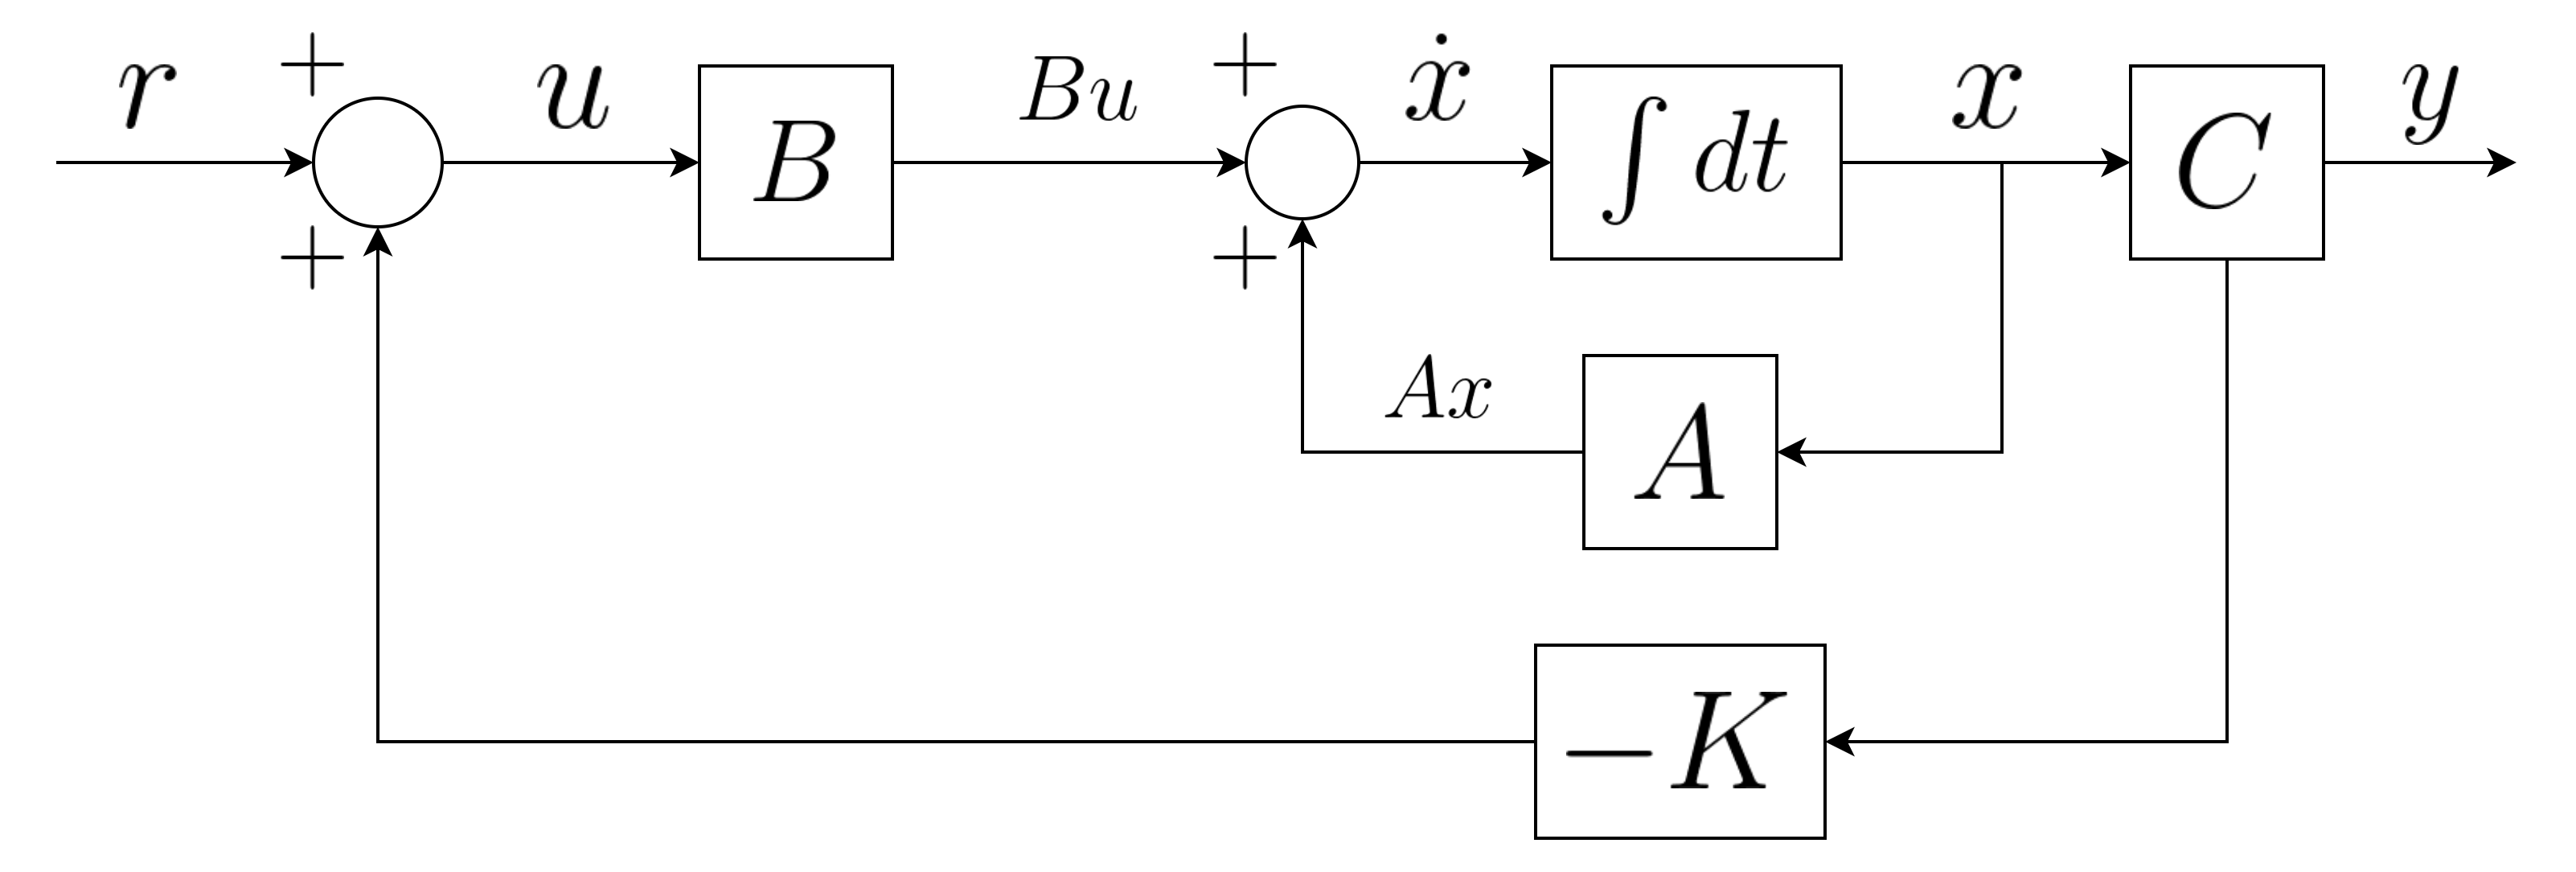
\includegraphics[width = 0.9\textwidth]{assets/image/homework_1.png}
                \caption{Diagram blok full state feedback pada state space}
                \label{gambar_1}
            \end{figure}
            Untuk mencari nilai K yang sesuai dengan sistem, dapat dilakukan dengan mencari persamaan karakteristik sistem sebagai berikut,
            \begin{equation}
                \begin{split}
                    \dot{x} &= Ax + Bu \\[5pt]
                    u &= -Kx + r \\[5pt]
                    \dot{x} &= Ax + B( -Kx + r) \\[5pt]
                    \dot{x} &= (A - BK)x + Br
                \end{split}
            \end{equation}
            \begin{equation}
                det(sI - (A - BK))
            \end{equation}
            \begin{equation}
                \begin{split}
                    \begin{bmatrix} \dot{x_1} \\ \dot{x_2} \\ \dot{x_3} \end{bmatrix} = \left( \begin{bmatrix} 0 & 1 & 0 \\ 0 & 0 & 1 \\ 0 & -20 & -12 \end{bmatrix} - \begin{bmatrix} 0 & 0 & 0 \\ 0 & 0 & 0 \\ K_1 & K_2 & K_3 \end{bmatrix} \right) \begin{bmatrix} x_1 \\ x_2 \\ x_3 \end{bmatrix} + \begin{bmatrix} 0 \\ 0 \\ 1 \end{bmatrix} r
                \end{split}
            \end{equation}
            \begin{equation}
                \begin{split}
                    0 &= det(sI - ( A - BK )) \\[5pt] 
                    0 &= \begin{vmatrix} s & -1 & 0 \\ 0 & s & -1 \\ K_1 & (20 + K_2) & s + (12 + K_3) \end{vmatrix}\\[5pt]
                    0 &= s^3 + (12 + K_3)s^2 + (20 + K_2)s + K_1
                    \label{persamaan_karakteristik}
                \end{split}
            \end{equation}
            Persamaan karakteristik sistem didapatkan pada persamaan \eqref{persamaan_karakteristik}. Untuk mengubah karakterisik sistem dapat dilakukan dengan memindahkan pole sistem. Pada analisis ini, pole sistem ditentukan bernilai $-1,-2$ dan $-3$. analisis pole sistem dapat dilihat pada persamaan \eqref{analisis_pole_sistem}. 
            \begin{equation}
                \begin{split}
                    pole &= [-1 -2 -3] \rightarrow (s+1)(s+2)(s+3) \\[5pt]
                    0 &= s^3 + 6s^2 + 11s + 6
                    \label{analisis_pole_sistem}
                \end{split}
            \end{equation}
            \begin{equation}
                \begin{split}
                    K_1 + 0 &= 6 \\[5pt] 
                    K_1 &= 6 - 0 \rightarrow K_1 = 6 \\[10pt]
                    K_2 + 20 &= 11 \\[5pt] 
                    K_2 &= 11 - 20 \rightarrow K_2 = -9 \\[10pt]
                    K_3 + 12 &= 6 \\[5pt] 
                    K_3 &= 6 - 12 \rightarrow K_3 = -6
                    \label{analisis_nilai_k_homework_1}
                \end{split}
            \end{equation}
            persamaan \eqref{persamaan_karakteristik} dan \eqref{analisis_pole_sistem} digunakan untuk menganalisis nilai $K$ pada sistem sebagaimana ditunjukkan pada persamaan \eqref{analisis_nilai_k_homework_1}. Hasil analisis menunjukkan nilai $K_1 = 6, K_2 = -9, K_3 = -6$. Untuk membuktikan kebenaran analisis matematis yang telah dilakukan, dibuat program untuk mencari nilai $K$ sebagai berikut,
            \lstinputlisting[language = Matlab]{assets/code/homework_1.m}
            Dari hasil program diatas didapatkan nilai $K_1, K_2$ dan $K_3$ yang \textbf{sama dengan hasil analisis secara matematis}. Program juga melakukan pengujian step pada sistem, hasil dari pengujian sistem menunjukkan karakteristik sistem yang tidak mengalami \textit{overshoot} namun memiliki waktu yang lama untuk mencapai \textit{steady state}. Hasil pengujian step sistem dapat dilihat pada Gambar \ref{gambar_2}. Hasil dari program dapat dilihat sebagai berikut,
            \lstinputlisting[language = Matlab]{assets/code/konsole_homework_1.m}
            \begin{figure}[H]
                \centering
                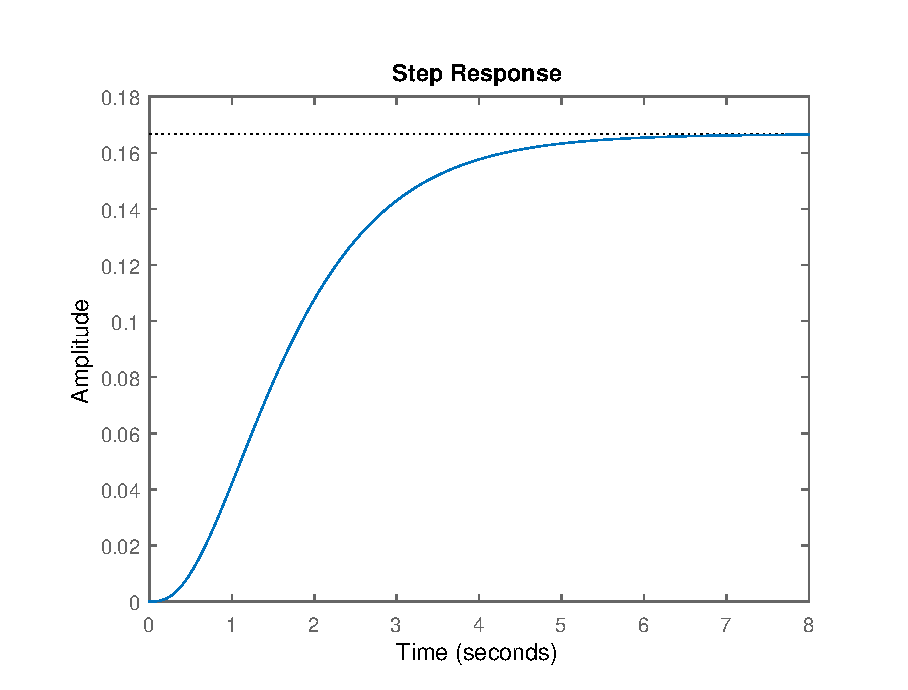
\includegraphics{assets/image/Homework_1.eps}
                \caption{hasil pengujian sistem sistem}
                \label{gambar_2}
            \end{figure}
        \subsection{Homework 2}
            Analisis yang dilakukan pada bagian ini adalah menggunakan metode pole placement untuk menghilangkan \textit{error steady state} pada sistem.
            \begin{equation}
                \dot{x_N} = e = r - Cx
            \end{equation}
            \begin{equation}
                \begin{split}
                    \begin{bmatrix} \dot{x} \\ \dot{x_N} \end{bmatrix} &= \begin{bmatrix} A & 0 \\ -C & 0 \end{bmatrix} \begin{bmatrix} x \\ x_N \end{bmatrix} + \begin{bmatrix} B \\ 0 \end{bmatrix} u + \begin{bmatrix} 0 \\ 1 \end{bmatrix} r \\[5pt]
                    y &= \begin{bmatrix} C & 0 \end{bmatrix} \begin{bmatrix} x \\ x_N \end{bmatrix}
                \end{split}
            \end{equation}
            \begin{equation}
                u = -Kx + K_E x_N \rightarrow = -\begin{bmatrix} K & K_E \end{bmatrix} \begin{bmatrix} x \\ x_N \end{bmatrix}
            \end{equation}
            \begin{equation}
                \begin{split}
                    \begin{bmatrix} \dot{x} \\ \dot{x_N} \end{bmatrix} &= \begin{bmatrix} (A-BK) & BK_E \\ -C & 0 \end{bmatrix} \begin{bmatrix} x \\ x_N \end{bmatrix} + \begin{bmatrix} 0 \\ 1 \end{bmatrix} r \\
                    y &= \begin{bmatrix} C & 0 \end{bmatrix} \begin{bmatrix} x \\ x_N \end{bmatrix}
                \end{split}
            \end{equation}
            dilakukan penambahan pole $s = -50$ pada sistem sebagai berikut,
            \begin{equation}
                \begin{split}
                    0 &= (s^3 + 28s + 192s + 640)(s + 50) \\[5pt]
                    0 &= s^4 + 78s^3 + 1592s^2 + 10240s + 32000
                    \label{persamaan_sistem_baru}
                \end{split}
            \end{equation}
            dari hasil penambahan pole dihasilkan persamaan sistem yang baruseperti yang ditunjukkan pada \eqref{persamaan_sistem_baru}. Persamaan karakteristik dianalisa sistem dapat dianalisis sebagai berikut,
            \begin{equation}
                \begin{split}
                    \begin{bmatrix} \dot{x} \\ \dot{x_N} \end{bmatrix} &= \begin{bmatrix} 0 & 1 & 0 & 0 \\ 0 & 0 & 1 & 0 \\ -K_1 & -(20 + K_2) & -(12 + K_3) & K_E \\ -1 & 0 & 0 & 0 \end{bmatrix}\begin{bmatrix} x \\ x_N \end{bmatrix} + \begin{bmatrix} 0 \\ 0 \\ 1 \end{bmatrix} r \\[10pt]
                    0 &= s^4 + (12 + K_3)s^3 + (20 + K_2)s^2 + K_1s + K_E
                    \label{persamaan_karaktersitik_homework_2}
                \end{split}
            \end{equation}
            dari persamaan \eqref{persamaan_sistem_baru} dan persamaan \eqref{persamaan_karaktersitik_homework_2} dapat dilakukan analisis nilai $K$ sistem sebagai berikut,
            \begin{equation}
                \begin{split}
                    K_E &= 32000 \\[10pt]
                    K_1 &= 10240 \\[10pt]
                    K_2 + 20 &= 1592 \\[5pt]
                    K_2 &= 10240 - 20 \rightarrow K_2 = 1572 \\[10pt]
                    K_3 + 12 &= 78 \\[5pt]
                    K_3 &= 78 - 12 \rightarrow K_3 = 66 \\[10pt]
                \end{split}
            \end{equation}
            dari hasil analisa matematis yang telah dilakukan didapatkan nilai $K$ sistem dengan $K_E = 32000, K_1 = 10240, K_2 = 1572, K_3 = 66$. Untuk memeriksa apakah nilai $K$ dari hasil analisis sistem dapat menghilangkan \textit{error steady state} pada sistem, dilakukan pengujian dengan Simulink MATLAB dengan membandingkan nilai $K$ sistem sebelumnya dengan nilai $K$ sistem hasil analisis matematis sebagai berikut,
            \begin{figure}[H]
                \centering
                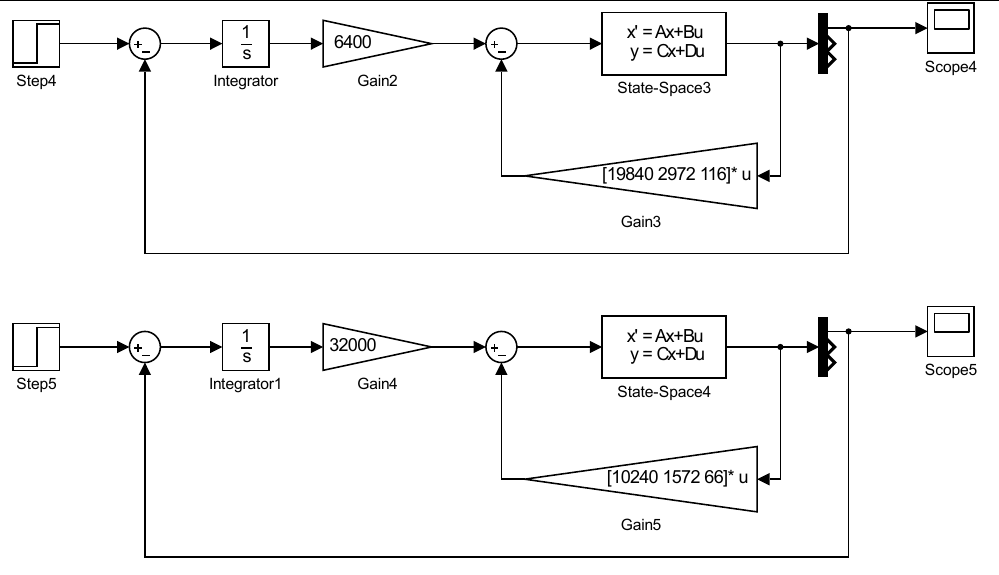
\includegraphics[width = \textwidth]{assets/image/simulink_homework_2.png}
                \caption{Diagram blok pengujian sistem}
                \label{gambar_3}
            \end{figure}
            Hasil pengujian yang telah dilakukan pada sistem dapat dilihat pada gambar \ref{gambar_4}. grafik dengan garis warna merah merupakan hasil dari sistem dengan nilai $K$ yang baru (hasil analisis matematis) sedangkan grafik garis warna biru menunjukkan hasil sistem dengan nilai $K$ yang lama. Dari hasil ini dapat dilihat bahwa sistem dengan nilai $K$ lama memiliki \textit{error steady state} sedangkan sistem dengan nilai $K$ yang baru tidak lagi memiliki \textit{error steady state}. Dapat disimpulkan bahwa pole placement dapat digunakan untuk menghilangkan \textit{error steady state}.
            \begin{figure}[H]
                \centering
                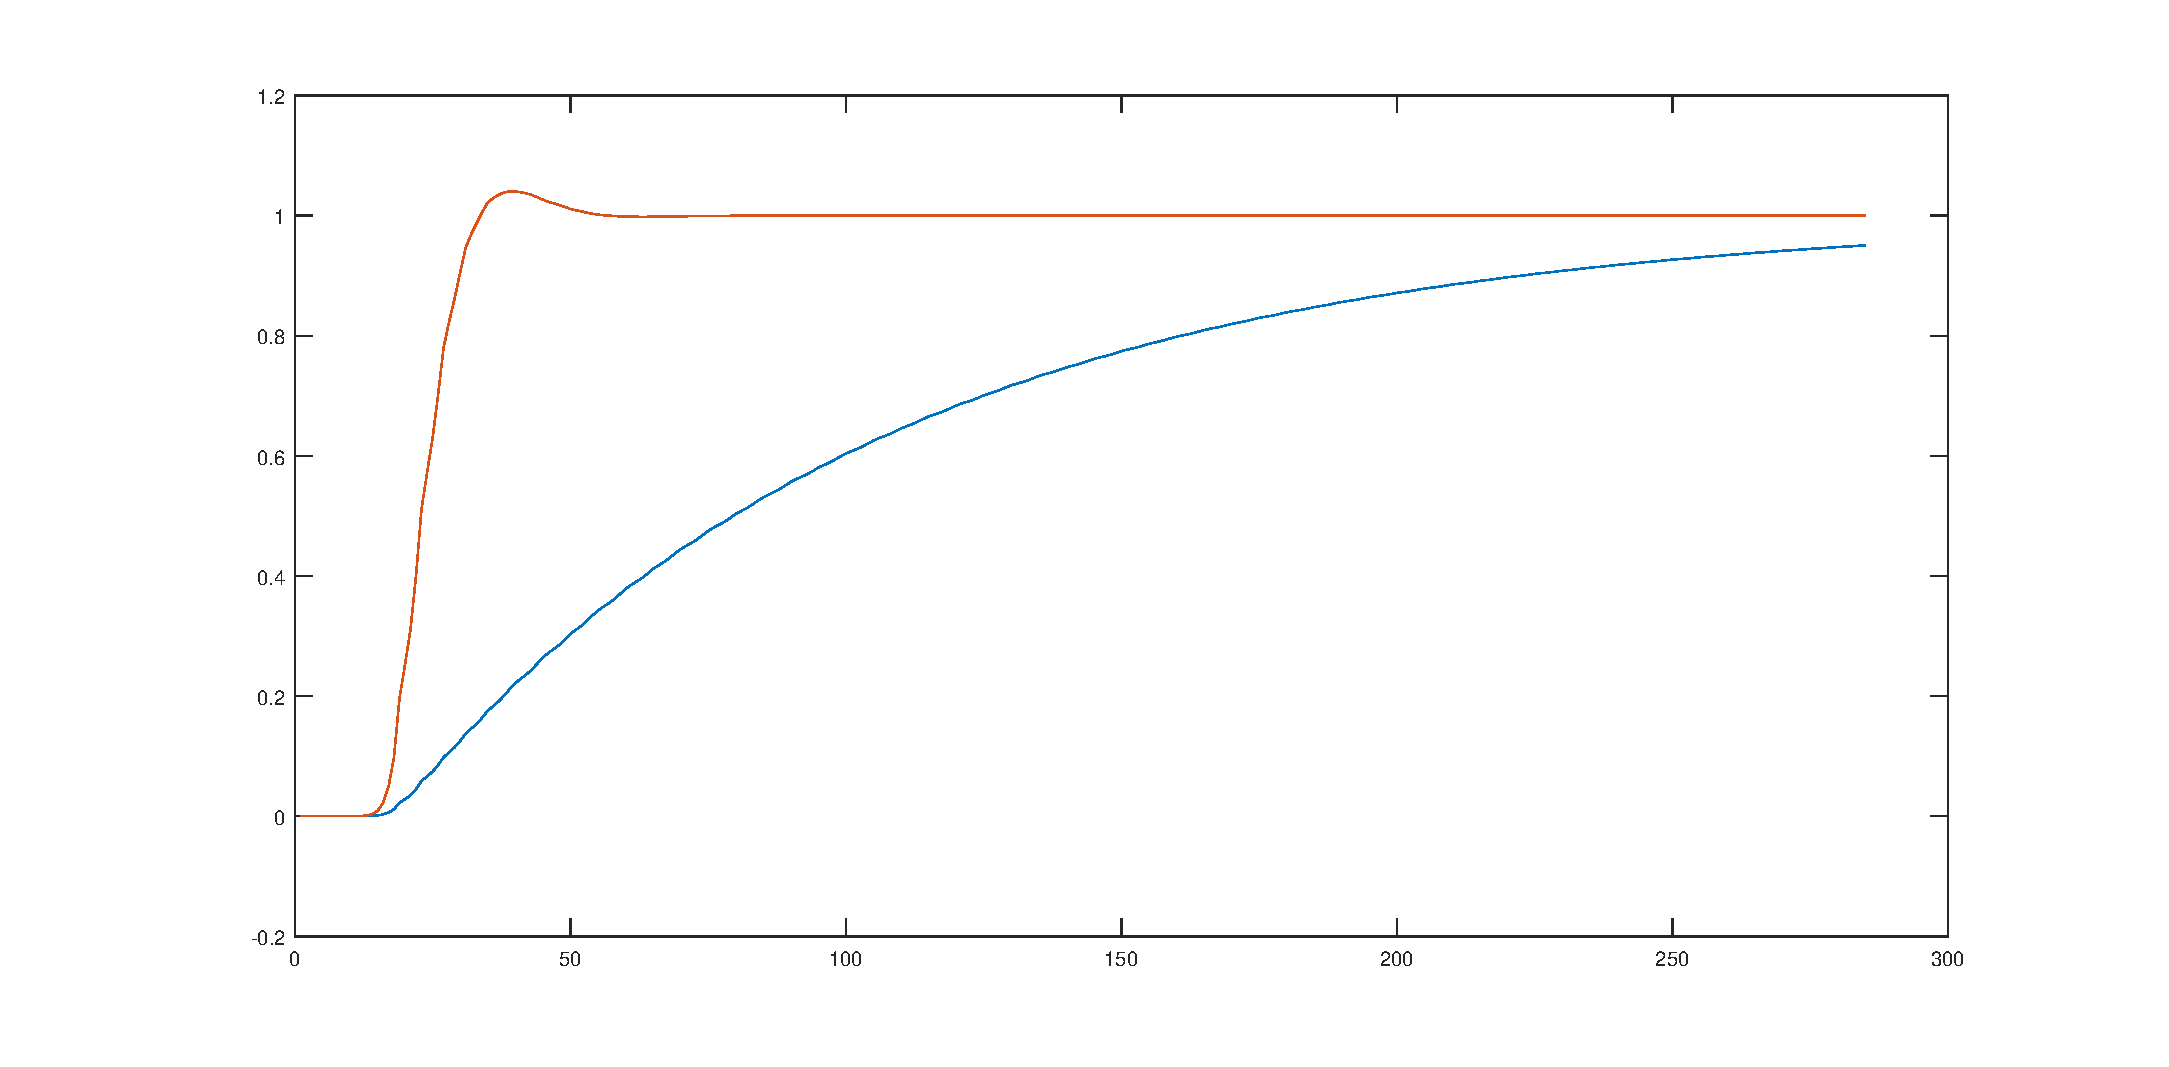
\includegraphics[width = \textwidth]{assets/image/Homework_2.eps}
                \caption{hasil pengujian performa sistem dengan metode state space untuk menghilangkan \textit{error steady state}}
                \label{gambar_4}
            \end{figure}
    \section{Kesimpulan}
        Dari hasil analisis dan pembahasan diatas diperoleh kesimpulan sebagai berikut,
        \begin{enumerate}
            \item Manipulasi karakteristik sistem dengan pole placement dapat dilakukan dengan menganalisis nilai $K$ pada sistem.
            \item \textit{Pole placement} merupakan metode yang dapat memanipulasi karakteristik sistem dengan memindahkan pole sistem. pole placement dapat digunakan dalam manipulasi sistem MIMO karena \textit{pole placement} dapat menggunakan sistem yang dimodelkan dengan \textit{state space}.
        \end{enumerate}
    \begin{thebibliography}{1}
        \bibitem[1]{Fahmizal} Fahmizal. 2020. "Pole Placement" dalam \textit{Modul Praktikum Teknik Kendali Lanjut} (hlm.1-9). Yogyakarta
    \end{thebibliography}
\end{document}